\section{\ddc{} Semantics}

The primitives of \ddc{} are deceptively simple.  Each captures a
simple concept, often familiar from type theory. However, in reality,
each primitive is multi-faceted. Each simultaneously describes a
collection of bit strings, two datatypes in the host language -- one
for the data representation (Rep) itself and one for its parse
descriptor (PD) -- and a transformation from bit strings into data and
corresponding meta-data. Moreover, the collection of bit strings
described need not be ``perfect'' --- many bit strings not exactly
matching the intuitive meaning of a type must also be successfully
parsed, with errors marked in the parse descriptor.

% Diagram:

% 011011101010101010000011...
%                 |
%                 |  [[ tau ]] _parser
%                 |
%                 v
%  [[tau]_pd  <-----------> [[ tau ]]_rep
%                 corr

What, then, are the semantics of a type? A number of factors went into
the design of \ddc{}, and they heavily influenced our choice for
the semantics of the calculus. First, it was necessary that the
calculus be simultaneously detailed enough to capture meaningful
differences between various data description languages (DDLs), 
and broad enough to express the constructs found in these languages.
Second, we sought to explain to DDL users the process by which
a bit stream is converted into an in-memory representation. For the
analyst, the data format already existed, with a specific meaning. We sought to precisely specify the transform so the
analyst knows how that meaning is mapped into the host language.
Finally, it was critical that \ddc{} include error reporting and
error handling mechanisms because errors are an intrinsic
characteristic of ad hoc data. 
%All DDLs are set up to handle errors with varying degrees of flexibility.
%   (warn the reader that the current calculus is not necessarily
%   ultimately flexible in this regard, but open to extension).

We therefore chose to specify the semantics of a type as the
transformation it performs on bit strings. From the formal
specification of a type's transformation - that is, parsing function,
we can infer all of the other properties mentioned above.  The
datatypes associated with the internal representation of the data and
its corresponding parse descriptor can be infered from the description
of the transformation itself. The set of ``perfect'' bit strings are
exactly those whose transformation results in a parse descriptor that
reports no errors.

\begin{table}
  \begin{center}
    \renewcommand{\arraystretch}{1.35}
    \begin{tabular}{l l}
      $\ddck[\ty,{\rctxt;\ctxt},\kind,\mcon]$ & {\it \ddc{}-type
        kinding}\\
      $\itsem[\ty] = \ity$ & {\it representation types of \ddc{} types}\\
      $\itpdsem[\ty] = \ity$ & {\it pd types of \ddc{} types}\\
      $\trans[\ty,\ctxt,\gk] = e$   & {\it \ddc{}-type semantics} \\
      $\kTrans[\gk,\ty] = \ity$     & {\it parser type} \\
      $\ptyc \rctxt = \ctxt$     & {\it context parser type}\\
      $\stsem[e,{\pctxt;\ctxt},\ity]$ & {\it \implang expression typing} \\
      $e \stepsto e'$ & {\it \implang expression evaluation}
    \end{tabular}
    \caption{Translations and Judgments}
    \label{tab:judg-list}
  \end{center}
\end{table}

In the remainder of this section, we formalize this semantics for \ddc{} types. 
For reference, we provide in \tblref{tab:judg-list} a listing of all the
judgments found in this section and a brief description of each. 

\begin{figure}[tp]
  \centering
  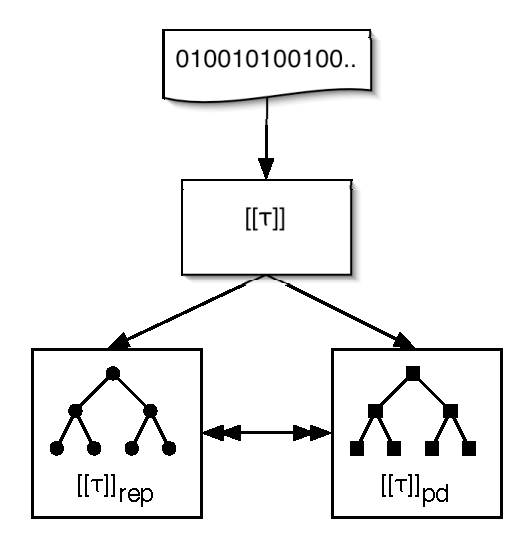
\includegraphics[height=2in,width=2in]{correspond}  
  \caption{Relationship between semantics judments}
  \label{fig:correspond-graphic}
\end{figure}

\subsection{Representations and Parse Descriptors}
\label{sec:intty-sem}
We now describe the exact correspondence between \ddc{} primitives and
data representations and parse descriptor \implang types. An
illustration of this correspondence is provided in
\figref{fig:correspond-graphic}.  The function $\trans[\ty,,]$ denotes
the parsing function for \ddc{}-type $\ty$. The functions
$\itsem[\ty]$ and $\itpdsem[\ty]$ denote the types of the Rep and PD,
respectively, output by the parsing function.

As \implang{} Rep and PD types belong to the host language, we now
introduce those types.

\begin{bnf}
  \name{Base Types} \meta{a} \::= 
  \iboolty \| \iintty \| \iunitty \| 
  \invty \nlalt \iecty \| \ioffty \| \ibitsty
  \\
  \name{Types} \meta{\ity} \::= 
      \ibasety \| \iarrow \ity \ity \| \iprod \ity \ity \|
      \isum \ity \ity \nlalt
      \iseq \ity \|
      \ierrty \ity \| \forall \ityvar.\ity  \| \ityvar \nlalt
      \imu \ityvar \ity   
\end{bnf}

{\em Define noval in this paragraph.}

The types include base types $a$, function types, product types (for
pairs), sum types (for injections), sequence types $\iseqty \ty$,
classifying sequences with element type $\ty$ and error types,
classifying tagged errors. In addition, we include parameterized types
$\forall \ityvar.\ity$ and type variables $\ityvar$ for polymorphism.
Finally, we have recursive types $\imu \ityvar \ity$.

\begin{figure}
\fbox{$\itsem[\ty] = \ity$}
\[
\begin{array}{lcl} 
\itsem[\ptrue] & = & \iunitty \\
\itsem[\pfalse] & = & \invty \\
\itsem[\pbase{e}] & = & \isum {\Irty(C)} \invty   \\
\itsem[\plam{\var}{\ity}{\ty}] & = & \itsem[\ty] \\
\itsem[\papp \ty e] & = & \itsem[\ty] \\
\itsem[\psig \var {\ty_1} {\ty_2}]  & = & \iprod {\itsem[\ty_1]} {\itsem[\ty_2]}    \\
\itsem[\psum {\ty_1} e {\ty_2}]     & = & \isum {\itsem[\ty_1]} {\itsem[\ty_2]} \\
\itsem[\pand {\ty_1} {\ty_2}]  & = & \iprod {\itsem[\ty_1]}{\itsem[\ty_2]}\\
\itsem[\pset x \ty e] & = & \isum {\itsem[\ty]}{\ierrty {\itsem[\ty]}}\\
% field names: length, elts
\itsem[\pseq \ty {\ty_{\text{sep}}} {\pterm e {\ty_{\text{term}}}}] & = & 
    \iprod \iintty {(\iseq{\itsem[\ty]})}             \\
%% \itsem[\pcase e c {\ty_1} {\ty_2}]       & = & \isum {\itsem[\ty_1]} {\itsem[\ty_2]}\\
\itsem[\ptyvar] & = & \ptyvar \\
\itsem[\pmu \ptyvar \ty] & = & \imu{\ptyvar}{\itsem[\ty]} \\
\itsem[\pcompute e \ity]                 & = & \ity \\
\itsem[\pabsorb \ty]                     & = & \isum \iunitty \invty \\
\itsem[\pscan \ty] & = & \isum {\itsem[\ty]} \invty 
%% \pext{
%% \itsem[\ptransform e e \ty]              & = & \itsem[\ty]\\
%% }
\end{array}
\]
\label{fig:rep-tys}
\caption{Representation Types}
\end{figure}

In Figure~\ref{fig:rep-tys}, we present the corresponding data
representation for each primitive of the \ddc{}. As our language
abstracts over base types, the corresponding internal types of base
types is based on the interface $\Irty$. As base type parses can fail,
producing no output, all base types correspond to a sum between the
actual type and the type $\invty$. The \ddc{} type $\ptrue$ always
succeeds while neither consuming nor producing data; hence it
corresponds to the $\iunitty$ type. Type $\pfalse$ always fails,
producing no data, and so corresponds to $\invty$.

As types can only be parameterized over expressions and expressions
are irrelevant to the simple types of the \implang{} language, type
abstraction and application can be ignored. Therefore, the internal
representation corresponding to a type application is exactly the
representation for the component type abstraction.  Similarly, the
representation for a type abstraction is the representation for the
underlying type. Note, however, that type abtractions can not directly
transform data - they must first be applied. Hence, the value of
assigning them any corresponding representation comes only from the
fact that we determine the representation type for application by
considering its component abstraction.

\ddc{} dependent products correspond to simple internal products.  \ddc{}
sums correspond to internal sums.
% ... additionally summing with the
% $\invty$ type to cover the possibility that neither type will be
% successfully parsed from the stream. Unlike products, we need to
% introduce the failure alternative for sums, as errors in both branches
% leaves us with no way to choose between the two erroneous values. With
% products, we have no need to choose between them; hence, if both
% branches have errors, we can return a pair of erroneous values. 
For intersection types, we would like access to the data in both forms
specified in the intersection.  Intersections therefore correspond to
a pair of values, one for each type. For set types, we wrap the
underlying element in an error in the event that the specified
constraint is not met. As we don't know at compile time whether the
constraint will be met by the data, the internal representation is a
sum. For sequences, we keep track of the length of the sequence as an
integer along with the sequence itself.

Recursive types generate recursive data structures, so the
\implang{}-language type corresponding to a recursive \ddc{} type is
just a recursive \implang{} type. Note that the \implang{} type uses the same
variable names as the \ddc{} type, and so the type corresponding to
the type variable $\ptyvar$ is exactly $\ityvar$.

The type corresponding to a computed expression is exactly the type of
the expression itself.  The type corresponding to absorb is either
$\iunitty$ when parsing the underlying type succeeds, or $\invty$,
when it fails. The type for scan is either that of the underlying
primitive, or $\invty$ to indicate that data matching that primitive
was not found.

Every parse descriptor consists of a header, which provides parse
information about the whole corresponding data structure and
subcomponents that are themselves parse descriptors, which describe
corresponding subcomponents of the data structure. Each header
contains an integer field recording the number of errors encountered
during parsing, an error code indicating the degree of success of the
parse -- success, success with errors, or failure -- and the span of
data described by the descriptor.  For brevity, we define an
abbreviation for the type of parse descriptor headers:
$\tyface{pd\_hdr} \triangleq \iintty \iprodi \iecty \iprodi \ispty$.

\begin{figure}
\fbox{$\itpdsem[\ty] = \ity$}
\[ 
\begin{array}{lcl} 
%% %% example: \ua.(int * a) + None
%% %%          pd = \ua.pd_hdr  * ((pd_hdr * ([int]_pd * [a]_pd)) + [None]_pd)
%% %%             = \ua.pd_hdr  * ((pd_hdr * ([int]_pd * a)) + [None]_pd)

\itpdsem[\ptrue] & = & \ipty \iunitty \\                                                  
\itpdsem[\pfalse] & = & \ipty \iunitty \\                                                  
\itpdsem[\pbase{e}] & = & \ipty \iunitty\\
\itpdsem[\plam \var \ity \ty] & = & \itpdsem[\ty] \\
\itpdsem[\papp \ty e] & = & \itpdsem[\ty] \\
\itpdsem[\psig \var {\ty_1} {\ty_2}] & = & 
               \ipty {\iprod {\itpdsem[\ty_1]} {\itpdsem[\ty_2]}} \\
\itpdsem[\psum {\ty_1} e {\ty_2}] & = & 
               \ipty {(\isum {\itpdsem[\ty_1]} {\itpdsem[\ty_2]})} \\
\itpdsem[\pand {\ty_1} {\ty_2}] & = & \ipty {\iprod {\itpdsem[\ty_1]} {\itpdsem[\ty_2]}}    \\
\itpdsem[\pset x \ty e] & = & \ipty {\itpdsem[\ty]} \\
\itpdsem[\pseq \ty {\ty_{\text{sep}}} {\pterm e {\ty_{\text{term}}}}] & = & 
  \iapty {\itpdsem[\ty]} \\
\itpdsem[\ptyvar] & = & \ptyvar \\
\itpdsem[\pmu \ptyvar \ty] & = & \imu \ptyvar {\itpdsem[\ty]} \\
\itpdsem[\pcompute e \ity]            & = & \ipty \iunitty \\
\itpdsem[\pabsorb \ty]                & = & \ipty \iunitty \\
\itpdsem[\pscan{\ty}] & = & \ipty {(\isum {(\iprod \iintty
    {\itpdsem[\ty]})} \iunitty)}
\end{array}
\]
\label{fig:pd-tys}
\caption{Parse Descriptor Types}
\end{figure}

In \figref{fig:pd-tys}, we present the corresponding parse
descriptor type for each \ddc{} type. The first three \ddc{}
primitives are all atomic, having no subcomponents. Therefore, they
require no more than a header. As with representation types, the
corresponding PD type of type constructors and type application is
that of their underlying type.  Dependent product, sum, and
intersection PD types are as expected.

Sequence parse descriptors contain a header and the parse descriptors
of all elements, but also include two additional fields - one
recording the total number of element errors, and one the sequence
length. Note that the number of element errors is distinct from the
number of sequence errors, as sequences can have errors that are not
related to any elements (such as errors reading separators).  We
introduce an abbreviation for array parse descriptor types,
$\iaptyname \; \ity \triangleq \iintty \iprodi \iintty \iprodi (\iseq
\ity)$.  We refer to the fields as \textit{neerr, length}, and
\textit{elts}.

The parse descriptor types for type variables and recursive types are
defined in the same way as for the data representations. We note,
additionally, that recursive types do not receive their own
header. {\em Should we explain this difference from other types?}
% which is critical for our iso-recursive treatment of recursive types
% (note that it would be even more so for an equi-recursive system).

Compute parse descriptors have no subelements, as the data they
describe is not parsed from the data source.  The absorb parse
descriptor type is unit in order to parallel the type of the
representation. We assume that just as the user does not want the rep
to be kept, so too the parse descriptor.  However, the absorb parse
descriptor does record a summary of the error information of its
underlying type.  Hence, if the underlying type had an error, then
absorb will report that an error occured. The scan parse descriptor is
either $\iunitty$, in case no match was found, or records the number
of bits skipped before the type was matched along with the type's
corresponding parse descriptor.

We conclude by specifying the \implang types of the parsers generated
from \ddc{} types in \figref{fig:parser-types}. Also included here is
the extension of parser type assignment to recursive contexts
$\rctxt$, decscribed in the next section. We note that the type for
parsers at kind $\kty$ corresponds to the diagram shown in
\figref{fig:correspond-graphic}. In essence, such a parser takes bits
as input and outputs a Rep and PD whose type is determined by the
\ddc{}-type from which the parser was generated.

\begin{figure}
\small
\fbox{$\kTrans[\gk,\ty] = \ity$} 
\fbox{$\ptyc{\rctxt} = \ctxt$} 
    
\begin{align*}
  %% Ty
  &\kTrans[\kty,\ty] = \extdom * \offdom \iarrowi \offdom * \itsem[\ty] * \itpdsem[\ty]
   \\
%%   \begin{semcasedef}{K-Abs}
%%     \kTrans[\gk_1 \-> \gk_2] = \kTrans[\gk_1] \-> \kTrans[\gk_2]
%%   \end{semcasedef}
%%    \\ \notag \\ 
   %% VAbs
   &\kTrans[\ity \iarrowi \gk,\ty] = \ity \iarrowi \kTrans[\gk,\ty]
\\
  &\ptyc{\cdot} = \cdot \\
  &\ptyc{\rctxt,\ptyvar{=}\pmu \ptyvar \ty} = \ptyc \rctxt,\codefont{f_\ptyvar}{:}
  \kTrans[\kty,\asub \rctxt {\pmu \ptyvar \ty}]
\end{align*}  
  \caption{Parser \Implang{} Types}
  \label{fig:parser-types}
\end{figure}

\subsection{\ddc{} Kinding}

% In essence, we
% need this well-formedness judgment to ensure two things: first, that
% type abstractions are applied to expressions of the correct type, and
% second, that higher-order primitives do not appear as direct subcomponents
% of basic primitives.

% The essential difference between type abstractions and basic types
% is that type constructors cannot directly describe a data source.
% They must always be fully applied first.  Therefore, we use the
% kinding system to differentiate between type constructors and ???
% types.  

\begin{figure}
\small
\fbox{$\ddck[\ty,\rctxt;\ctxt,\kind,\mcon]$} 

$\infer[True]{
    \ddck[\ptrue,\rctxt;\ctxt,\kty,\con]
  }{\wfd {} \ctxt}
$
$\quad \infer[False]{
    \ddck[\pfalse,\rctxt;\ctxt,\kty,\con]
  }{\wfd {} \ctxt}
$
$\quad \infer[Const]{
    \ddck[\pbase{e},\rctxt;\ctxt,\kty,\con]
  }{
    \begin{semcond}
      \stsem[e,\cdot;\ctxt,\ity] &
      (\vlet {\ity \iarrowi \kty} {\Ikind(C)})
    \end{semcond}
  }
$
$\quad \infer[Abs]{
    \ddck[\plam{\var}{\ity}{\ty},
         \rctxt;\ctxt,\ity \iarrowi \kind,\mcon]
  }{
    \ddck[\ty,\rctxt;\ectxt{\var{:}\ity},\kind,\mcon]
  }
$
$\quad \infer[App]{
    \ddck[\papp{\ty}{e},\rctxt;\ctxt,\gk,\mcon]
  }{
    \ddck[\ty,\rctxt;\ctxt,\ity \iarrowi \gk,\mcon] &
    \stsem[e,\cdot;\ctxt,\ity]
  }
$
$\quad \infer[Prod]{
    \ddck[\psig{x}{\ty}{\ty'},\rctxt;\ctxt,\kty,\con]
  }{       
    \begin{semcond}
      \ddck[\ty,\rctxt;\ctxt,\kty,\mcon]\\
      \ddck[\ty',\rctxt;
             \ectxt {x{:}\iprod {\itsem[\asub \rctxt \ty]} 
               {\itpdsem[\asub \rctxt \ty]}},
             \kty,\mcon']
    \end{semcond}
  }
$
$\quad
  \infer[Sum]{
    \ddck[\psum{\ty}{e}{\ty'},\rctxt;\ctxt,\kty,\con]
  }{
    \ddck[\ty,\rctxt;\ctxt,\kty,\mcon] & \ddck[\ty',\rctxt;\ctxt,\kty,\mcon'] 
  }
$
$\quad
  \infer[Intersection]{
    \ddck[\pand \ty {\ty'},\rctxt;\ctxt,\kty,\con]
  }{
    \ddck[\ty,\rctxt;\ctxt,\kty,\mcon] & \ddck[\ty',\rctxt;\ctxt,\kty,\mcon'] 
  }
$
$\quad
  \infer[Set]{
    \ddck[\pset x \ty e,\rctxt;\ctxt,\kty,\con]
  }{ 
    \ddck[\ty,\rctxt;\ctxt,\kty,\mcon] & 
    \stsem[e,\cdot;
    \ectxt{x{:}\iprod{\itsem[\asub \rctxt \ty]} 
      {\itpdsem[\asub \rctxt \ty]}},\iboolty]
  }
$
$\quad
  \infer[Seq]{
    \ddck[\pseq \ty {\ty_s} {\pterm e {\ty_t}},\rctxt;\ctxt,\kty,\con]
  }{
    \begin{array}{c}
    \ddck[\ty,\rctxt;\ctxt,\kty,\mcon] \qquad
    \ddck[{\ty_s},\rctxt;\ctxt,\kty,\mcon_s] \qquad
    \ddck[{\ty_t},\rctxt;\ctxt,\kty,\mcon_t] \\
    \stsem[e,\cdot;\ctxt,
    \iprod {\itsem[{\ty_m}]}      
    {\itpdsem[{\ty_m}]}
    \iarrowi \iboolty]
    \quad (\ty_m = \asub \rctxt {\pseq \ty {\ty_s} {\pterm e {\ty_t}}})
    \end{array}
  }
$
$\quad
  \infer[Var]{
    \ddck[\ptyvar,{\rctxt;\ctxt},\kty,\ncon]
  }{\wfd {} \ctxt \quad \ptyvar \in \dom \rctxt}
  \quad
  \infer[Rec]{
    \ddck[\pmu \ptyvar \ty,\rctxt;\ctxt,\kty,\con]
  }{
    \ddck[\ty,{\rctxt,\ptyvar {=} \pmu \ptyvar \ty;\ctxt},\kty,\con]
  }
$
$\quad
  \infer[Compute]{       
    \ddck[\pcompute{e}{\ity},\rctxt;\ctxt,\kty,\con]
  }{
    \stsem[e,\cdot;\ctxt,\ity]
  }      
$
$\quad
  \infer[Absorb]{
    \ddck[\pabsorb{\ty},\rctxt;\ctxt,\kty,\con]
  }{
    \ddck[\ty,\rctxt;\ctxt,\kty,\mcon]
  }
$
$\quad
  \infer[Scan]{
    \ddck[\pscan{\ty},\rctxt;\ctxt,\kty,\con]
  }{
    \ddck[\ty,\rctxt;\ctxt,\kty,\mcon]
  }
$ 
\caption{\ddc{} Kinding Rules}
\label{fig:ddc-kinding}
\end{figure}

The kinding judgment defined in \figref{fig:ddc-kinding} determines
well-formed \ddc{} types, assigning kind $\kty$ to basic types and
$\ity \iarrowi \kind$ to type abstractions. There are two contexts in
which the kinding judgment is made. First appears $\rctxt$, an ordered
list of mappings between type variables and recursive types.
\[
\rctxt \mathrel{::=} \cdot \bnfalt \rctxt,\ptyvar{=}\pmu \ptyvar \ty
\]
This context serves two purposes: first, to ensure the well-formedness
of types with free type variables, as in rule~${Var}$, and, second, to
provide mappings between recursive type variables and their associated
type. Due to this second purpose, we also consider a context $\rctxt$
to be a substitution from type variables to types. Application of such
substitutions has the form $\asub \rctxt \ty$, as show in rules
$Prod$, $Set$ and $Seq$.

The second context is an unordered set that binds expression variables
to their types and has the familiar form:
\[
\ctxt \mathrel{::=} \cdot \bnfalt \ctxt,{\var{:}\ty}
\]

Due to the inclusion of recursive types, one aspect of well
formedness is that we cannot allow types such as $\pmu \ptyvar
\ptyvar$. More generally, we need to ensure (for well formed types) that
recursive type variables are separated from their binder by at least
one basic primitive, a condition which we call {\it contractiveness}.
Therefore, we additionally annotate every judgment with a contractiveness
indicator, which can be one of $\con$, $\ncon$, or $\mcon$. The use of
$\con$ indicates that the type is contractive, while $\ncon$,
indicates that it is not and $\mcon$ indicates that it may be either
one. We also assign an ordering to $\mcon$ of $\ncon < \con$. 

Otherwise, the rules are mostly straightforward. We highlight here
just two of them. Base types, $\pbase{e}$, are assigned a kind from
the interface $\Ikind$.  {\em Is $\Ikind$ and interface itself or is
  it just a function within the base-type interface?} While their kind
does not differentiate them from type abstractions, they are not well
formed when not applied.  Also note that, once applied, all base types
have kind $\kty$. The product rule shows that $\var$ is bound as a
pair of a representation and a corresponding parse descriptor. Note
that $\rctxt$ is applied to the type before translation to a
\implang{} type - thereby closing it - as open \ddc{} types do not
translate into well formed \implang{} types.

\subsection{\Implang{} Language}

\begin{figure}[tp]
\small
\begin{bnf}
  \name{Variables} \meta{f,x,y} \\

  \name{Bit}   \meta{b}   \::= 0 \| 1 \\ 
  \name{Bits}  \meta{B}   \::= \vec{b} \\ 
  \name{Constants} \meta{c} \::=
      () \| \itrue \| \ifalse \| 0 \| 1 \| -1 \| \dots \nlalt
      \ierr \| \data \| \off \| \iok \| \iecerr \| \ldots \\

  \name{Values} \meta{v,r,p} \::= 
      \const \| % \ilam{\nrm \var}{\ity}{e} \| 
      \ifun {\nrm f} {\nrm x} e \nlalt
      \ipair v v \| \iinld{\ity}{v} \| \iinrd{\ity}{v} \nlalt
      \iarr{\vec{v}} \| \ierror{v} \\

  \name{Operators} \meta{op} \::= 
      = \; \| \; < \; \| \inotop \| \isizeofop
      \| \ldots \\

  \name{Expressions} \meta{e} \::= 
      \const \| \var \| \iop{e} \nlalt
%      \ilam {\nrm \var} \ity e \| 
      \ifun {\nrm f} {\nrm x} e \| 
      \iapp e e \nlalt
%      \iletfun {\nrm f} {\nrm x} e \; \iin \; e' \| 
      \ilet {\nrm x} e \; e \nlalt
      \iif e \; \ithen e \; \ielse e \nlalt
      \ipair{e}{e} \| \ipi {\nrm i}{e} \nlalt
      \iinld{\ity}{e} \| \iinrd{\ity}{e} \nlalt
      \icaseg{e}{\nrm x}{e}{\nrm x}{e} \nlalt
      \iarr{\vec e} \| \iappend e e \| \isub e {\nrm e} \nlalt
      \ierror{e} \| \iexamine{e}      
\end{bnf}
\caption{\Implang{} Language}
\label{fig:implang-syntax}
\end{figure}

In \figref{fig:implang-syntax} we introduce an extension of the
simple-typed polymorphic lambda calculus for two purposes. First,
while the \ddc{} is not tied to any particular expression language, we
present this calculus as an example of a potential expression
language.  It captures many of the features found in common expression
languages at a high level. Second, we will later encode the parsing
semantics of the \ddc{} in this calculus.

{\em Rewrite this next paragraph.}

Most of the syntax is taken unchanged from standard presentations of
the polymorphic lambda calculus. The major differences are in the
constants. As this language is used to encode parsing functions, we
include bits and offsets as atomic elements of the calculus. While the
parsers may manipulate individual bits of source data, they more often
manipulate whole sources at once, here represented by bit strings
$\idata$. 
The constants $c$ include the unit value, the standard boolean values
and the integers. In addition, we include abstract bit string offsets
$\off$, $\ierr$, used to indicate unrecoverable errors in the data
source (at the level of base types), and error codes $\iok$ and $\iecerr$.

The operators include the standard boolean operators and integer
comparisons. We also have a special $\isizeofop$ operator that returns
the size in the data source of a variable. Operators are distinct from
constants, as the operator implementations are not necessarily written
in the \implang language.  Expressions include constants $\const$,
variables (denoted by any of the metavariables $f,x,y$), recursive
functions $\ifun {\nrm f} {\nrm x} e$, let expressions, conditionals,
pairs, projections, injections, cases expressions, an arbitrary length
(possible zero) sequence $\iarr{\vec e}$, sequence append $\iappend e
{e'}$, and sequence indexing $\isub e {\nrm i}$. In addition, we add a
new expression $\ierror e$, which wraps $e$ in an error tag, and
$\iexamine e$, which strips error tags off of error values in order to
look at the underlying value.

Finally, we introduce some syntactic sugar and abbreviations for use
throughout the paper. Unnamed functions $\ilam {\nrm x} \ity e$ are
equivalent to $\ifun {\nrm f} {\nrm x} e$, with $f \not\in {\rm
  FV}(e)$ and function bindings $\iletfun {\nrm f} {\nrm x} e \; \iin
\; e'$ are equivalent to $\ilet {\nrm f} {\ifun {\nrm f} {\nrm x} e}
\; e'$.  We define the type abbreviation $\ispty$ to be a pair of
offsets, $\iprod \ioffty \ioffty$. Also, as sums and products are
binary operators, we introduce the convention that a multi-type sum or
product should be converted into binary sums and products by
considering the operators to be right associative. Hence, for example,
$a \iprodi b \iprodi c$, should be read as $a \iprodi (b \iprodi c)$.

We define standard judgments for the static semantics
($\stsem[e,{\pctxt;\ctxt},\ity]$) and operational semantics ($e
\stepsto e'$) of the \implang{} language. For further details, please
see our companion technical report~\cite{fisher+:pads-semantics-ext}.

\subsection{Parsing Semantics of the \ddc{}}
\label{sec:parse-sem}

The semantics of a type is a function, expressed in the \implang
language that parses bit strings to produce data structures in the
lambda calculus.  Each parsing function takes a data source and an
offset in the data source and returns a new offset, a representation
of the parsed data (Rep) and a parse descriptor (PD). The semantics of
each type is show in \figref{fig:ddc-sem}. Note that the semantics
function is partial and only guaranteed to translate well-formed PADS
types.

In the definitions below, we use $\lampair{\codefont e}$ as an
abbreviation for $\ilam{\ivar}{}{
  \ilet B {\ipi{1}{\ivar}}\;
  \ilet \off {\ipi{2}{\ivar}}\; e}$.
% $ \sfn{x}{}{( \sfn{B}{}{
%     \sfn{\off}{}{\mathtt{e}} }) \sapp (\spi{1}{\ivar}) \sapp
%   (\s) }$ 
and,similarly, $\ilet {\itup{\off,r,p}} e$ as an abbreviation for
$\ilet \var e$ followed by a serious of let expressions binding the
variables from the pattern to the appropriate projections from $\var$.
We define the parsers with respect to a set of Rep and PD constructors
$\mathtt{R_{tyname}, P_{tyname}}$, defined in \figref{fig:cons-funs},
a set of assorted built-in functions defined in
Appendix~\ref{sec:asst-functions}, and the base-type implementations
$\Iimp$.

For every type, there are two aspects to parsing: the mechanics of
parsing and the tracking of errors that occur during the parse.
Roughly speaking, the error tracking is handled by the constructor
functions, while the mechanics of the parsing appears in the function
body.

{\em When should we discuss the workings of the constructors? Should
  they be inlined or discussed separately?}

The semantics of $\ptrue$ and $\pfalse$ show that they do not parse
any data - that is, they do not advance the input stream. A look at
their constructors shows that the parse descriptor for $\ptrue$ always
indicates no errors, while that of $\pfalse$ always indicates one
error. The semantics of base types merely applies the implementation
of the base type's parser to the appropriate arguments. Abstraction
and application are defined directly in terms of \implang language
abstraction and application.  Dependent pairs read the first element
at $\off$ and then the second at $\off'$, the offset returned from
parser of the first element.  Notice that we bind the pair of the
returned representation and parse descriptor to the variable $x$
before parsing the second element, as $x$ is bound by the dependent
product. Finally, we combine the results using the constructor
functions, returning $\off''$ as the final offset of the parse.

Sums first attempt to parse according to the left type, returning its
value if it parses without errors. Otherwise, it parses according to
the right type. Intersections read both types starting at the same
point. They advance the stream to the maximum of the two offsets
returned by the component parsers. The construction of the parse
descriptor is similar to that of products. For set types, we call the
parser for the underlying type $\ty$, bind $r$ and $p$ to $\var$, and
then check whether the result satisfies the specified constraint $e$.
We construct the representation and parse descriptor based on the
result of this check. Note, however, that we advance the stream
independent of whether the constraint was satisfied.

Sequences have the most complicated semantics. Unlike other types,
sequences do not contain a predefined number of subcomponents. Rather,
that number depends on a combination of the data, the termination
predicate and termanator type. Therefore, the sequence parser uses
recursive functions to implement this open-ended semantics. The first
function defined in the parser, named $\codefont{isDone}$, is a
predicate that checks whether the parser should terminate. It first
checks whether the end of the source has been reached, then whether
the termination condition $e$ has been satisfied, and, finally,
whether the terminator type can be read from the stream, without
errors, at $\off$.

The next function, $\codefont{continue}$, is the heart of the parser. It
takes four arguments - two offsets, a sequence representation and a
sequence parse descriptor.  The two offsets are the starting and
ending offset of the previous round of parsing.  First, the function
checks whether these offsets are equal, in order to determine whether
the parser made progress in its last parsing operation. This check is
critical in ensuring that the parser terminates. Next, the parser
checks whether the sequence should be terminated. The first check is
not placed in the $\codefont{isDone}$ function, as $\codefont{isDone}$ is not always
called after a parsing operation, as will be seen below. If either of
these checks succeed then the function terminates.  Otherwise, we
attempt to read a separator followed by an element and then continue
parsing the sequence, calling $\codefont{continue}$ again with the results.

Next, we create an initial sequence Rep and PD. Before we commence
parsing, we check whether the sequence is empty, calling
$\codefont{isDone}$. If not, then we read an element and create a new
representation and parse descriptor for the sequence.  Note that we
use the PD for $\ptrue$ in place of a separator PD, as
no separator is read before the first element.  Finally, we continue
reading the sequence with a call to $\codefont{continue}$.

Recursive types are translated into recursive functions with a special
function name corresponding to the name of the bound type variable. A
recursive type variable is translated directly into this special name.
We note that the body of the recursive function is somewhat more complicated
than is strictly necessary for the purposed of semantics. Instead, we
could have chosen to define it as follows:
\[
  \trans[\pmu \ptyvar \ty,,] = \ifun {f_\ptyvar} {\itup{\data,\off}} 
  {\trans[\ty,,] \; \itup{\data,\off}}
\]
However, we define it as shown in \figref{fig:ddc-sem}, for the
purpose of simplifying the meta-theory. For details, please see our
companion technical report.

The definition of $\kwd{compute}$ just calls the compute constructors. The
Rep constructor returns the value computed by
$e$, while the PD records no errors and reports a span of
length 0, as no data is consumed by the computation. The $\kwd{absorb}$
parser first parses the underlying type and then calls the absorb
constructors, passing only the PD, which is needed by the
Rep constructor to determine whether an error occured while
parsing the underlying type. If so, the value returned is a
$\ierr$. Otherwise, it is $\iunitty$.

The semantics of the $\kwd{scan}$ type is to attempt to parse the underlying
type from the stream at an increasing scan-offset, $i$, from the original
offset $\off$,  until success is achieved
or a predefined maximum scan-offset (\cd{scan\_max}) is reached. Note
that, upon success, $i$ is passed to the PD constructor function,
which both records it in the PD and sets the error code based on
it. It is considered a regular error for the value to be found at a
positive $i$, whereas it is a panic error for it not to be found at
all.

\begin{figure}
\small
\fbox{$\trans[\ty,\ctxt,\gk] = e$} 

\begin{itemize}
\renewcommand{\labelitemi}{}
%% None 
\item $\trans[\ptrue,\ctxt,\kty] =
  \lampair{\spair<\off,\newrep{true}{},\newpd{true}{\off}>}$

%% False 
\item $\trans[\pfalse,,] =
  \lampair{\spair<\off,\newrep {false}{},\newpd {false}{\off}>}$

%% Const 
\item $\trans[\pbase{e},\ctxt,\kty] =
  \lampair{\iapp {\iapp {\Iimp(C)} (e)} {\itup {\idata,\off}}}$

%% Abs 
\item $\trans[\plam{\var}{\ity}{\ty},,] =
   \sfn{\nrm\var}{\ity}{\trans[\ty,\ectxt{\var{:}\ity},\kind]}$

%% App 
\item $\trans[\papp{\ty}{e},\ctxt,\gk] =
  \trans[\ty,,] \sapp e$

%% Prod 
\item $\trans[\psig{x}{\ty}{\ty'},\ctxt,\kty] =$ \\
  $\begin{array}{l}  
    \lampair{} \\
    \quad  \ilet {\spair<\off',r,p>} 
    {{\trans[\ty,,]} \sapp \spair<\idata,\off>} \\
    \quad  \ilet x {\ictup{r,p}}\\
    \quad  \ilet {\spair<\off'',r',p'>} 
    {{\trans[\ty',,]} \sapp \spair<\idata,\off'>} \\
    \quad \spair<\off'',\newrep {\gS}{r,r'},\newpd {\gS}{p,p'}>
  \end{array}$

%% Sum 
\item $\trans[\psum{\ty}{e}{\ty'},,] =$ \\
  $\begin{array}{l}  
  \lampair{} \\
  \quad \ilet {\itup{\off',r,p}}{\trans[\ty,,] \sapp \spair<\idata,\off>} \\
  \quad \iif {\pdok p} \; \ithen {
    \def \r {\newrep {+left}{r}}
    \def \p {\newpd {+left}{p}}
    \spair<\off',\r,\p>} \\
  \quad \ielse {\ilet {\itup{\off',r,p}}{\trans[\ty',,] \sapp \spair<\idata,\off>}} \\
  \quad 
  {  % begin scope
    \def \r {\newrep {+right}{r}}
    \def \p {\newpd {+right}{p}}
    %% 
    \spair<\off',\r,\p>
  }\\ % end scope
  \end{array}$

%% Intersection 
\item $\trans[\pand{\ty}{\ty'},,] =$ \\
  $\begin{array}{l}  
     \lampair{} \\
     \quad \ilet {\itup{\off',r,p}} {\trans[\ty,,] \sapp \spair<\idata,\off>} \\
     \quad \ilet {\itup{\off'',r',p'}} {\trans[\ty',,] \sapp \spair<\idata,\off>} \\
     \quad {\spair<\codefont{max}(\off',\off''),\newrep {\&}{r,r'},\newpd {\&}{p,p'}>}
   \end{array}$

%% Set 
\item $\trans[\pset{x}{\ty}{e},\ctxt,\kty] =$ \\
  $\begin{array}{l}  
    \lampair{} \\
    \quad \ilet {\itup{\off',r,p}}{\trans[\ty,,] \sapp \spair<\idata,\off>} \\
    \quad \ilet x {\ictup{r,p}}\\
    \quad \ilet c e \\
    \quad \spair<\off',\newrep {set} {c,r},\newpd {set} {c,p}>
  \end{array}$
% \end{itemize}
% \caption{\ddc{} Semantics}
% \label{fig:ddc-sem}
% \end{figure}
% \begin{figure}
% \small
% \begin{itemize}
% \renewcommand{\labelitemi}{}
%% Array 
\item $\trans[\pseq{\ty}{\ty_s}{\pterm e {\ty_t}},,] =$ \\
  $\begin{array}{l}  
    \lampair{}\\
      \quad \iletfun {isDone}{\itup{\off,r,p}}{\\
        \qquad \ior {\eofpred {\idata,\off}} {e\codefont {\sapp
          \spair<r,p>}} \iori \\
        \qquad \ilet {\itup{\off',r',p'}}{\trans[\ty_t,,] \spair<\idata,\off>}\\
        \qquad \pdok{p'}
      }\\
      \quad \iin \\
      \quad \iletfun {continue} {\itup{\off,\off',r,p}} {\\
        \qquad \iif  {\off = \off' \iori \isdone {\off',r,p}} \; \ithen {\itup{\off',\codefont{r,p}}} \\
        \qquad \ielse {
          \ilet {\itup{\off_s,r_s,p_s}}{\trans[\ty_s,,] \sapp \spair<\idata,\off'>}}\\
        \qquad \ilet {\itup{\off_e,r_e,p_e}}{\trans[\ty,,] \sapp \ictup{\idata,\off_s}}\\
        \qquad \mathtt{continue} \sapp \ictup{
            \off,\off_e,\newrep {seq} {r,r_e}, \newpd {seq} {p, p_s, p_e}
        }}\\
      \quad \iin
   \end{array}$\\
  $\begin{array}{l}  
      \quad \ilet {\mathtt{r}} {\newrep {seq\_init}{}}\\
      \quad \ilet {\mathtt{p}} {\newpd {seq\_init}{\off}}\\
      \quad \iif {\isdone{\off,r,p}} \; \ithen {\itup{\off,\codefont{r,p}}}\\
      \quad \ielse {\ilet {\itup{\off_e,r_e,p_e}}{\trans[\ty,,] \sapp
          \spair<\idata,\off>}} \\
      \quad \mathtt{continue} \sapp \ictup{\off,\off_e,
        \newrep {seq} {r,r_e}, \newpd {seq} {p, \newpd {true} \off, p_e}}      
  \end{array}$

%% Var
\item $\trans[\ptyvar,,] = \codefont{f_\ptyvar}$

%% Mu
\item $\trans[\pmu \ptyvar \ty,,] =$ \\
  $\begin{array}{l}
  \ifun {f_\ptyvar} {\itup{\data,\off}} {}\\
  \quad \ilet {\itup{\off',r,p}} 
  {\trans[\ty,,] \iappi \ictup{\data,\off}} \\
  \qquad \ictup{\off',r,p}   
  \end{array}$

%% Compute
\item $\trans[\pcompute e \ity,,] =$ \\
  $\lampair{\itup{\off,\newrep {compute} {\nrm e},\newpd {compute} \off}}$

%% Absorb
\item $\trans[\pabsorb \ty,,] =$ \\
  $\begin{array}{l}  
    \lampair{}\\
    \quad \ilet {\itup {\off',r,p}} {\trans[\ty,,] \sapp \spair<\idata,\off>}\\
    \quad \itup{\off',\newrep {absorb} p,\newpd {absorb} p}   
  \end{array}$

%% Scan
\item $\trans[\pscan \ty,,] =$ \\
  $\begin{array}{l}  
    \lampair{}\\
    \quad \iletfun {try} {i} {\\
      \qquad \ilet {\itup{\off',r,p}} {\trans[\ty,,] \sapp
        \codefont{\spair<\data,\off + i>}} \\
      \qquad \iif {\pdok p}\; \ithen {\ictup{\off',\newrep {scan} r,
        \newpd {scan} {i,p}}}\; \ielse {}\\
      \qquad \iif {\codefont{i = scanMax}}\; \ithen {\ictup{\off,\newrep {scan\_err} {},
        \newpd {scan\_err} {\off}}}\; \ielse {}\\
      \qquad \codefont {try \sapp (i+1)}
   }\\
   \quad \iin \\
   \qquad \codefont{try \sapp 0}
  \end{array}$
\end{itemize}
%\caption{\ddc{} Semantics (cont.)}
\caption{\ddc{} Semantics}
\label{fig:ddc-sem}
\end{figure}

\begin{figure}
\small
\begin{itemize}
\renewcommand{\labelitemi}{}

\item %[True:]
\item $\ifun {R_{true}} \iuval \iuval$
\item $\ifun {P_{true}} \off {\itup{\itup{0,\iok,\ipair \off \off},\iuval}}$

\item %[False:]
\item $\ifun {R_{false}} \iuval \ierr$
\item $\ifun {P_{false}} \off ((1,\iecpc,\ipair \off \off),())$

\item %[Pair:]
\item $\ifun {R_{\gS}} {\ipair {r_1} {r_2}} {\itup {\codefont{r_1,r_2}}}$
\item $\ifun{H_{\gS}} {\ictup{h_1,h_2}}{}$ \\
  $\begin{array}{l}
    \ilet {nerr} {\codefont{pos \; \itup{{h_1}.{nerr} + {h_2}.{nerr}}}}\\
    \ilet {ec} {\codefont{ecCeil} \iappi \codefont{h_1.ec} \iappi \codefont{h_2.ec}} \\
    \ilet {sp} {\ictup{h_1.sp.begin, h_2.sp.end}} \\
    \quad \ictup {nerr,ec,sp}
  \end{array}$

\item $\ifun {P_{\gS}} {\ictup{p_1, p_2}} {\ictup {H_{\gS} \itup{p_1.h,p_2.h},\itup{p_1,p_2}}}$

\item %[Sum:]
\item $\ifun {R_{+left}} r {\iinl {\codefont r}}$
\item $\ifun {R_{+right}} r {\iinr {\codefont r}}$

\item $\ifun {H_+} h {\ictup{pos(h.nerr),h.ec,h.sp}}$
\item $\ifun {P_{+left}} p {\ictup{\codefont{H_+} \iappi p.h, \iinl p}}$
\item $\ifun {P_{+right}} p {\ictup{\codefont{H_+} \iappi p.h, 
      \iinr  p}}$

\item %[Intersection:]
\item $\ifun {R_{\&}} {\ictup {r,r'}} {\ictup {r,r'}}$
\item $\ifun {H_{\&}} {\ictup {h_1, h_2}} {}$ \\
    $\begin{array}{l}
      \ilet {nerr} {\codefont{pos \; \itup{{h_1}.{nerr} + {h_2}.{nerr}}}}\\
      \ilet {ec} {\codefont{ecCeil} \iappi \codefont{h_1.ec} \iappi \codefont{h_2.ec}} \\
      \ilet {sp} {\ictup{h_1.sp.begin, max \itup{h_1.sp.end, h_2.sp.end}}} \\
      \quad \ictup {nerr,ec,sp}
    \end{array}$

\item $\ifun {P_{\&}} {\ictup {p_1,p_2}} {\ictup{H_{\&} \iappi 
      \itup{p_1.h, p_2.h},\itup{p_1,p_2}}}$

\item %[Set:]
\item $\ifun {R_{set}} {\ictup{c,r}} {
    \iif {\codefont c} \; \ithen {\iinl {\codefont r}} \; \ielse {\iinr {\ierror
        {\codefont r}}}
  }$ 
\item $\ifun {P_{set}} {\ictup {c, p}} {}$ \\
    $\begin{array}{l}
      \iif {\codefont c} \; \ithen {\ictup{(pos(p.nerr),p.ec,p.sp),p}} \\
      \ielse {\ictup {(pos(1+p.nerr),\iecerr,p.sp),p}}
    \end{array}$
% \end{itemize}
% \caption{Constructor Functions}
% \label{fig:cons-funs}
% \end{figure}
% \begin{figure}
% \small
% \begin{itemize}
% \renewcommand{\labelitemi}{}

\item %[Array:] 
\item $\ifun {R_{seq\_init}} {\iuval} {\ictup{0,\ieseq}}$   
\item $\ifun {P_{seq\_init}} \off {\ictup{(0,\iok,\ipair \off
      \off),(0,0,\ieseq)}}$

\item $\ifun {R_{seq}} {\ictup{r, r_e}} 
  {\ictup{r.len+1,\iappend{r.elts} {\iarr{r_e}}}}$
\item $\ifun {H_{seq}} {\ictup{h, h_s, h_e}} {}$ \\
  $\begin{array}{l}
      \ilet {eerr} {
        \codefont{\iif {h.neerr = 0 \mathrel{and} h_e.nerr > 0}}\\
        \codefont{\quad \ithen 1 \;  \ielse 0}
      }\\
      \ilet {nerr} {\codefont{h.nerr + pos(h_s.nerr) + eerr}}\\
      \ilet {ec} {\codefont{\iif{nerr = 0}\; \ithen {\iok}\; \ielse
          \iecerr}} \\
      \ilet {sp} {\ictup{h.sp.begin,h_e.sp.end}} \\
      \quad \ictup {nerr,ec,sp}
    \end{array}$

\item $\ifun{P_{seq}} {\ictup{p, p_s, p_e}}{}$ \\ 
  $\begin{array}{l}
    \codefont{(H_{seq} \iappi \itup{p.h,p_s.h,p_e.h},}\\ 
    \codefont{\itup{p.neerr + pos(p_e.nerr), p.len + 1,\iappend {p.elts}
        {\iarr{p_e}}})}
  \end{array}$

\item %[Compute:]
\item $\ifun{R_{compute}} r {\codefont r}$
\item $\ifun{P_{compute}} \off {\ictup{\itup{0,\iok,\ipair \off \off},\iuval}}$

\item %[Absorb:]
\item $\ifun {R_{absorb}} p {\iif {\pdok p}\; 
    \ithen {\iinl \iuval}\; \ielse {\iinr \ierr}}$
\item $\ifun {P_{absorb}} p {\ictup{p.h,\iuval}}$

\item %[Scan:]
\item $\ifun{R_{scan}} r  {\codefont{\iinl r}}$
\item $\ifun{P_{scan}} {\itup{i,p}} {}$ \\
$\begin{array}{l}
\ilet {nerr} {\codefont{pos(i + p'.nerr)}}\\
\ilet {ec} {\iif {\codefont{nerr = 0}}\; \ithen \iok\; \ielse \iecerr} \\
\ilet {hdr} {\ictup{nerr,ec,(p.sp.begin - i,p.sp.end)}} \\
\quad \ictup{hdr,\iinl {\ictup{i,p}}}
\end{array}$

\item $\ifun {R_{scan\_err}} {()} {\iinr \ierr}$
\item $\ifun {P_{scan\_err}} \off {\ilet {hdr} {\ictup{1,pc,(\off,\off)}}}$\\
  \verb+ +$\ictup{hdr,\iinr \iuval}$

%% \item[Transform:]
%% \item \fnm{P_T} (h,b) = (h,(???,b))
\end{itemize}
\caption{Constructor Functions}
\label{fig:cons-funs}
%\caption{Constructor Functions (cont.)}
\end{figure}

\clearpage

%%% Local Variables: 
%%% mode: latex
%%% TeX-master: "semantics"
%%% End: 
